% Options for packages loaded elsewhere
\PassOptionsToPackage{unicode}{hyperref}
\PassOptionsToPackage{hyphens}{url}
%
\documentclass[
  8pt,
  ignorenonframetext,
  aspectratio=43,
]{beamer}
\usepackage{pgfpages}
\setbeamertemplate{caption}[numbered]
\setbeamertemplate{caption label separator}{: }
\setbeamercolor{caption name}{fg=normal text.fg}
\beamertemplatenavigationsymbolsempty
% Prevent slide breaks in the middle of a paragraph
\widowpenalties 1 10000
\raggedbottom
\setbeamertemplate{part page}{
  \centering
  \begin{beamercolorbox}[sep=16pt,center]{part title}
    \usebeamerfont{part title}\insertpart\par
  \end{beamercolorbox}
}
\setbeamertemplate{section page}{
  \centering
  \begin{beamercolorbox}[sep=12pt,center]{part title}
    \usebeamerfont{section title}\insertsection\par
  \end{beamercolorbox}
}
\setbeamertemplate{subsection page}{
  \centering
  \begin{beamercolorbox}[sep=8pt,center]{part title}
    \usebeamerfont{subsection title}\insertsubsection\par
  \end{beamercolorbox}
}
\AtBeginPart{
  \frame{\partpage}
}
\AtBeginSection{
  \ifbibliography
  \else
    \frame{\sectionpage}
  \fi
}
\AtBeginSubsection{
  \frame{\subsectionpage}
}
\usepackage[]{noto-sans}
\usepackage{amssymb,amsmath}
\usepackage{ifxetex,ifluatex}
\ifnum 0\ifxetex 1\fi\ifluatex 1\fi=0 % if pdftex
  \usepackage[T1]{fontenc}
  \usepackage[utf8]{inputenc}
  \usepackage{textcomp} % provide euro and other symbols
\else % if luatex or xetex
  \usepackage{unicode-math}
  \defaultfontfeatures{Scale=MatchLowercase}
  \defaultfontfeatures[\rmfamily]{Ligatures=TeX,Scale=1}
\fi
\usetheme[]{ScaDS}
\usecolortheme{dolphin}
% Use upquote if available, for straight quotes in verbatim environments
\IfFileExists{upquote.sty}{\usepackage{upquote}}{}
\IfFileExists{microtype.sty}{% use microtype if available
  \usepackage[]{microtype}
  \UseMicrotypeSet[protrusion]{basicmath} % disable protrusion for tt fonts
}{}
\makeatletter
\@ifundefined{KOMAClassName}{% if non-KOMA class
  \IfFileExists{parskip.sty}{%
    \usepackage{parskip}
  }{% else
    \setlength{\parindent}{0pt}
    \setlength{\parskip}{6pt plus 2pt minus 1pt}}
}{% if KOMA class
  \KOMAoptions{parskip=half}}
\makeatother
\usepackage{fancyvrb}
\usepackage{xcolor}
\IfFileExists{xurl.sty}{\usepackage{xurl}}{} % add URL line breaks if available
\IfFileExists{bookmark.sty}{\usepackage{bookmark}}{\usepackage{hyperref}}
\hypersetup{
  pdftitle={Activity Prediction using Dynamic Graph Embeddings},
  pdfauthor={Jens Petit},
  hidelinks,
  pdfcreator={LaTeX via pandoc}}
\urlstyle{same} % disable monospaced font for URLs
\VerbatimFootnotes % allow verbatim text in footnotes
\newif\ifbibliography
\usepackage{color}
\usepackage{fancyvrb}
\newcommand{\VerbBar}{|}
\newcommand{\VERB}{\Verb[commandchars=\\\{\}]}
\DefineVerbatimEnvironment{Highlighting}{Verbatim}{commandchars=\\\{\}}
% Add ',fontsize=\small' for more characters per line
\newenvironment{Shaded}{}{}
\newcommand{\AlertTok}[1]{\textcolor[rgb]{1.00,0.00,0.00}{\textbf{#1}}}
\newcommand{\AnnotationTok}[1]{\textcolor[rgb]{0.38,0.63,0.69}{\textbf{\textit{#1}}}}
\newcommand{\AttributeTok}[1]{\textcolor[rgb]{0.49,0.56,0.16}{#1}}
\newcommand{\BaseNTok}[1]{\textcolor[rgb]{0.25,0.63,0.44}{#1}}
\newcommand{\BuiltInTok}[1]{#1}
\newcommand{\CharTok}[1]{\textcolor[rgb]{0.25,0.44,0.63}{#1}}
\newcommand{\CommentTok}[1]{\textcolor[rgb]{0.38,0.63,0.69}{\textit{#1}}}
\newcommand{\CommentVarTok}[1]{\textcolor[rgb]{0.38,0.63,0.69}{\textbf{\textit{#1}}}}
\newcommand{\ConstantTok}[1]{\textcolor[rgb]{0.53,0.00,0.00}{#1}}
\newcommand{\ControlFlowTok}[1]{\textcolor[rgb]{0.00,0.44,0.13}{\textbf{#1}}}
\newcommand{\DataTypeTok}[1]{\textcolor[rgb]{0.56,0.13,0.00}{#1}}
\newcommand{\DecValTok}[1]{\textcolor[rgb]{0.25,0.63,0.44}{#1}}
\newcommand{\DocumentationTok}[1]{\textcolor[rgb]{0.73,0.13,0.13}{\textit{#1}}}
\newcommand{\ErrorTok}[1]{\textcolor[rgb]{1.00,0.00,0.00}{\textbf{#1}}}
\newcommand{\ExtensionTok}[1]{#1}
\newcommand{\FloatTok}[1]{\textcolor[rgb]{0.25,0.63,0.44}{#1}}
\newcommand{\FunctionTok}[1]{\textcolor[rgb]{0.02,0.16,0.49}{#1}}
\newcommand{\ImportTok}[1]{#1}
\newcommand{\InformationTok}[1]{\textcolor[rgb]{0.38,0.63,0.69}{\textbf{\textit{#1}}}}
\newcommand{\KeywordTok}[1]{\textcolor[rgb]{0.00,0.44,0.13}{\textbf{#1}}}
\newcommand{\NormalTok}[1]{#1}
\newcommand{\OperatorTok}[1]{\textcolor[rgb]{0.40,0.40,0.40}{#1}}
\newcommand{\OtherTok}[1]{\textcolor[rgb]{0.00,0.44,0.13}{#1}}
\newcommand{\PreprocessorTok}[1]{\textcolor[rgb]{0.74,0.48,0.00}{#1}}
\newcommand{\RegionMarkerTok}[1]{#1}
\newcommand{\SpecialCharTok}[1]{\textcolor[rgb]{0.25,0.44,0.63}{#1}}
\newcommand{\SpecialStringTok}[1]{\textcolor[rgb]{0.73,0.40,0.53}{#1}}
\newcommand{\StringTok}[1]{\textcolor[rgb]{0.25,0.44,0.63}{#1}}
\newcommand{\VariableTok}[1]{\textcolor[rgb]{0.10,0.09,0.49}{#1}}
\newcommand{\VerbatimStringTok}[1]{\textcolor[rgb]{0.25,0.44,0.63}{#1}}
\newcommand{\WarningTok}[1]{\textcolor[rgb]{0.38,0.63,0.69}{\textbf{\textit{#1}}}}
\usepackage{graphicx}
\makeatletter
\def\maxwidth{\ifdim\Gin@nat@width>\linewidth\linewidth\else\Gin@nat@width\fi}
\def\maxheight{\ifdim\Gin@nat@height>\textheight\textheight\else\Gin@nat@height\fi}
\makeatother
% Scale images if necessary, so that they will not overflow the page
% margins by default, and it is still possible to overwrite the defaults
% using explicit options in \includegraphics[width, height, ...]{}
\setkeys{Gin}{width=\maxwidth,height=\maxheight,keepaspectratio}
% Set default figure placement to htbp
\makeatletter
\def\fps@figure{htbp}
\makeatother
\setlength{\emergencystretch}{3em} % prevent overfull lines
\providecommand{\tightlist}{%
  \setlength{\itemsep}{0pt}\setlength{\parskip}{0pt}}
\setcounter{secnumdepth}{-\maxdimen} % remove section numbering
\usepackage{caption}
\captionsetup[figure]{labelformat=empty}
\usepackage{cmbright}
\ifluatex
  \usepackage{selnolig}  % disable illegal ligatures
\fi

\title{Activity Prediction using Dynamic Graph Embeddings}
\author{Jens Petit}
\date{2020-10-29}

\begin{document}
\frame{\titlepage}

\begin{frame}{Outline}
\protect\hypertarget{outline}{}
\tableofcontents
\end{frame}

\hypertarget{graph-representation-learning}{%
\section{Graph Representation
Learning}\label{graph-representation-learning}}

\begin{frame}{Graph Representation Learning}
\protect\hypertarget{graph-representation-learning-1}{}
Test
\end{frame}

\hypertarget{dynamic-graph-representation-learning}{%
\section{Dynamic Graph Representation
Learning}\label{dynamic-graph-representation-learning}}

\begin{frame}{Dynamic Graph Representation Learning}
\protect\hypertarget{dynamic-graph-representation-learning-1}{}
\begin{block}{Discrete-time dynamic graphs (DTDG)}
\protect\hypertarget{discrete-time-dynamic-graphs-dtdg}{}
Sequences of static graph snapshots.
\end{block}

\begin{block}{Continuous-time dynamic graphs (CTDG)}
\protect\hypertarget{continuous-time-dynamic-graphs-ctdg}{}
Timed list of events, including node addition, deletion and edge
addition and deletion.
\end{block}
\end{frame}

\begin{frame}{Temporal Graph Networks (TGN)}
\protect\hypertarget{temporal-graph-networks-tgn}{}
\begin{figure}
\centering
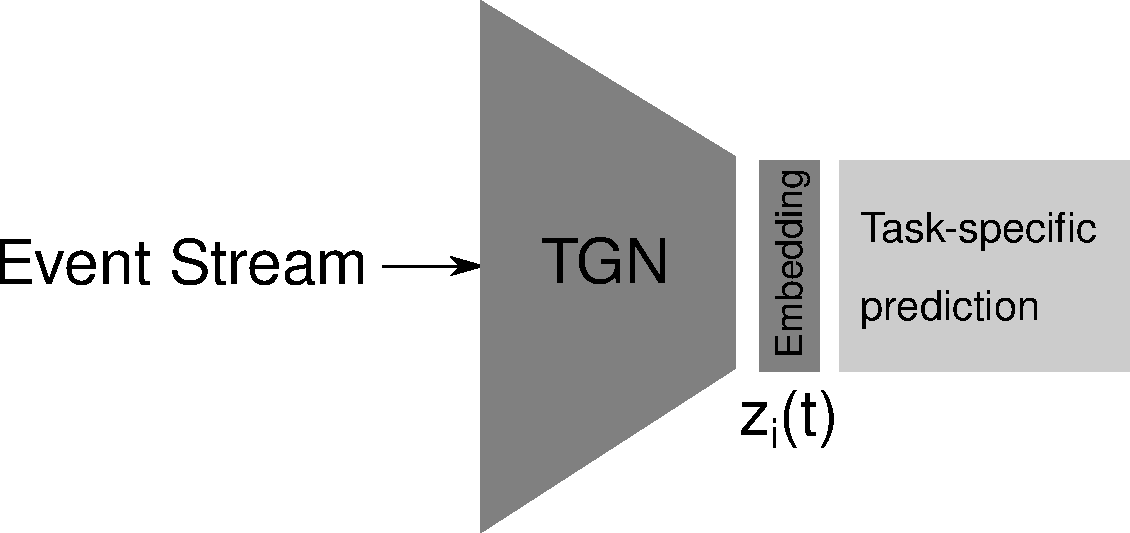
\includegraphics[width=0.65\textwidth,height=\textheight]{tgn_general.pdf}
\caption{The city of Leipzig as a graph}
\end{figure}

Current decoders:

\begin{itemize}
\tightlist
\item
  future edge (`link') prediction
\item
  dynamic node classification
\end{itemize}

Problem settings:

\begin{itemize}
\tightlist
\item
  Transductive: only nodes which have been used in training
\item
  Inductive: additionally nodes which have \emph{not} been used in
  training
\end{itemize}
\end{frame}

\begin{frame}{Example: TGN for future link prediction\footnote<.->{``Temporal
  Graph Networks For Deep Learning on Dynamic Graphs, \emph{Rossi et
  al.}''}}
\protect\hypertarget{example-tgn-for-future-link-prediction1}{}
Datasets:

\begin{itemize}
\tightlist
\item
  Reddit, Wikipedia: Bipartite interaction graphs with users and
  subreddits/pages as nodes.
\item
  Twitter: Users are nodes and retweets are interactions.
\end{itemize}

All interaction events carry text features (tweets, edits, posts) and
70\%-15\%-15\% (train-valid-test) chronological split is used.

Exemplary decoder: simple MLP decoder mapping from the concatenation of
two node embeddings to the probability of the edge
\end{frame}

\begin{frame}[fragile]{Example: TGN encoder}
\protect\hypertarget{example-tgn-encoder}{}
\begin{figure}
\centering
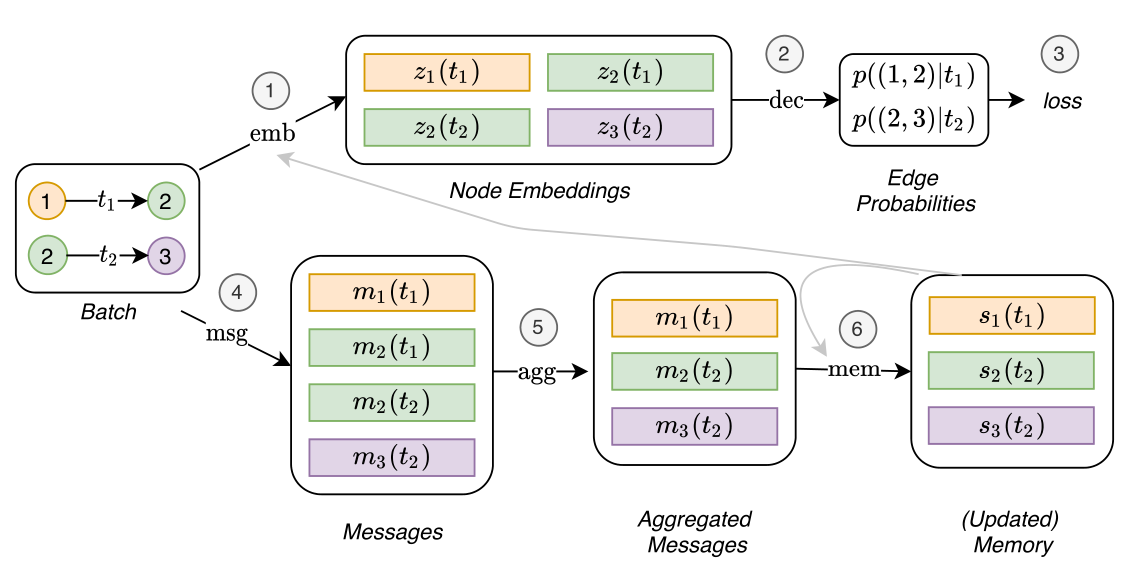
\includegraphics[width=0.65\textwidth,height=\textheight]{tgn_computations.png}
\caption[TGN computations on a single batch of time-stamped
interactions.]{TGN computations on a single batch of time-stamped
interactions\footnotemark{}.}
\end{figure}
\footnotetext{Figure taken from ``Temporal Graph Networks For Deep
  Learning on Dynamic Graphs, \emph{Rossi et al.}''

  \hypertarget{gdelt-dataset}{%
  \section{GDELT Dataset}\label{gdelt-dataset}}

  \hypertarget{the-gdelt-dataset}{%
  \subsection{The GDELT Dataset}\label{the-gdelt-dataset}}

  \begin{quote}
  ``The GDELT Project monitors the world's broadcast, print, and web
  news from nearly every corner of every country in over 100 languages
  and identifies the people, locations, organizations, themes, sources,
  emotions, counts, quotes, images and events driving our global society
  every second of every day, creating a free open platform for computing
  on the entire world.''
  \end{quote}

  \begin{itemize}
  \tightlist
  \item
    Global Knowledge Graph
  \item
    Global Event Database
  \item
    Global Entity Graph
  \item
    Global Frontpage Graph
  \end{itemize}

  \hypertarget{the-global-entity-graph}{%
  \subsection{The Global Entity Graph}\label{the-global-entity-graph}}

  Random sample of news articles every 15 minutes (roughly 100k per day)

  Google NLP API extracts entities from each article

\begin{Shaded}
\begin{Highlighting}[]
\FunctionTok{\{}
  \DataTypeTok{"url"}\FunctionTok{:} \StringTok{"https://chicago.suntimes.com/news/washington{-}state{-}ends{-}racially{-}biased{-}death{-}penalty/"}\FunctionTok{,}
  \DataTypeTok{"lang"}\FunctionTok{:} \StringTok{"en"}\FunctionTok{,}
  \DataTypeTok{"date"}\FunctionTok{:} \StringTok{"2018{-}10{-}12T00:15:00Z"}\FunctionTok{,}
  \DataTypeTok{"score"}\FunctionTok{:} \FloatTok{{-}0.2}\FunctionTok{,}
  \DataTypeTok{"magnitude"}\FunctionTok{:} \FloatTok{12.3}\FunctionTok{,}
  \DataTypeTok{"entities"}\FunctionTok{:} \OtherTok{[}
    \FunctionTok{\{}
      \DataTypeTok{"name"}\FunctionTok{:} \StringTok{"Supreme Court"}\FunctionTok{,}
      \DataTypeTok{"type"}\FunctionTok{:} \StringTok{"ORGANIZATION"}\FunctionTok{,}
      \DataTypeTok{"numMentions"}\FunctionTok{:} \DecValTok{1}\FunctionTok{,}
      \DataTypeTok{"avgSalience"}\FunctionTok{:} \FloatTok{0.04405}
    \FunctionTok{\}}\OtherTok{,}
    \ErrorTok{...}
\ErrorTok{\}}
\end{Highlighting}
\end{Shaded}

  \hypertarget{creating-a-graph}{%
  \subsection{Creating a Graph}\label{creating-a-graph}}

  Each pair of entities occurring in a single article correspond to an
  edge event with timestamp:

\begin{Verbatim}
Nathan Trott        RB Leipzig
Manchester United   RB Leipzig
West Ham            RB Leipzig
Timo Werner         RB Leipzig
Ralf Rangnick       RB Leipzig
Bundesliga          RB Leipzig
Patrick Dempsey     Leipzig
Leipzig             Germany
Patrick Dempsey     Leipzig
Leipzig             Germany
Patrick Dempsey     Leipzig
Leipzig             Germany
...
\end{Verbatim}

  Restricting to the 4 most salient entities gives roughly 200k edges
  per day

  \hypertarget{data-example-ipcc}{%
  \subsection{Data Example: IPCC}\label{data-example-ipcc}}

  \begin{columns}[T]
  \begin{column}{0.48\textwidth}
  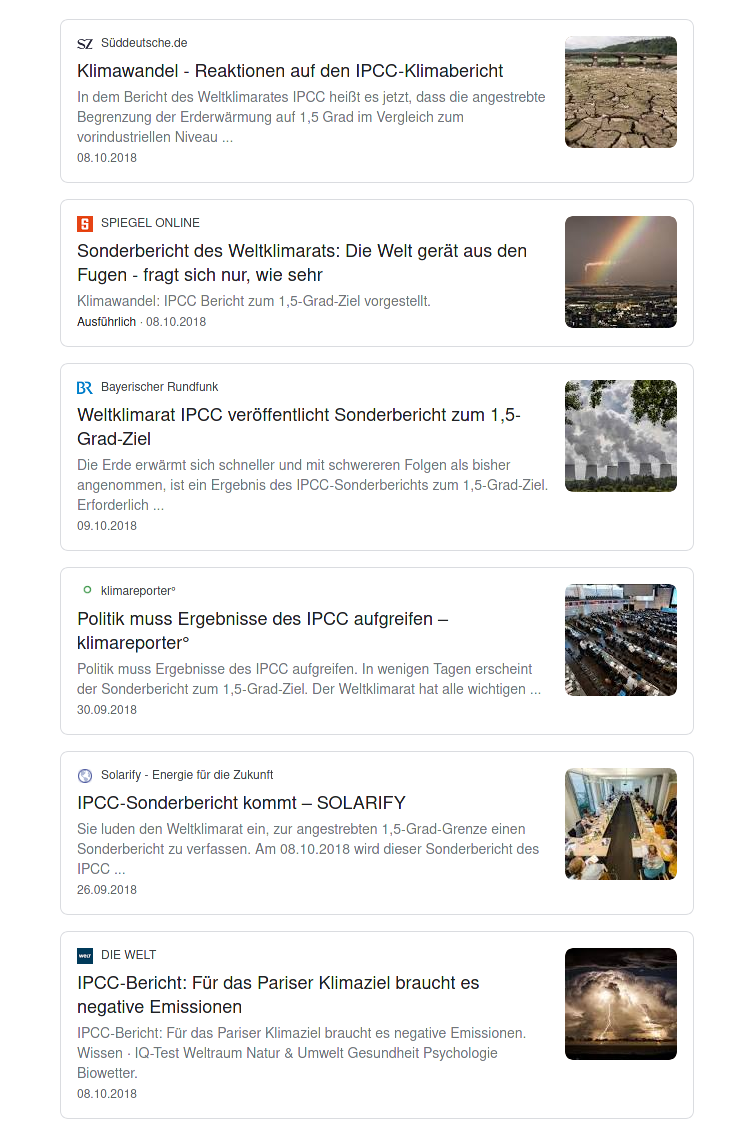
\includegraphics{ipcc_headlines.png}
  \end{column}

  \begin{column}{0.48\textwidth}
  \begin{figure}
  \centering
  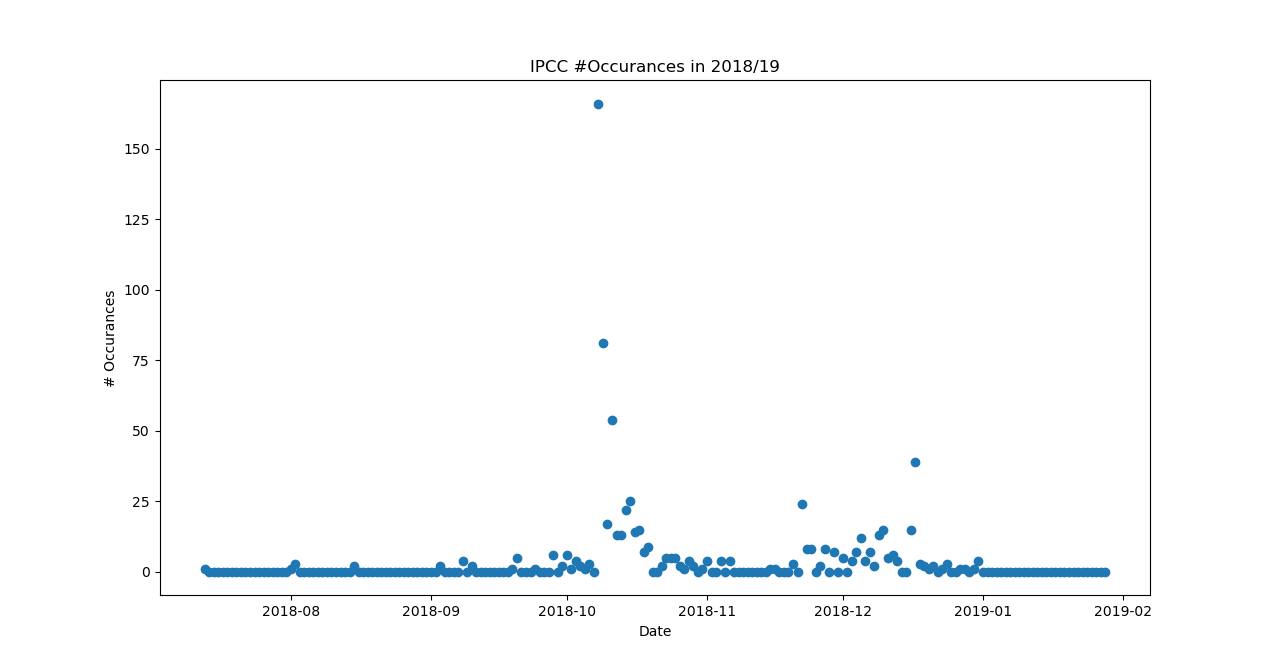
\includegraphics{ipcc_2018.png}
  \caption{\# Occurrences IPCC}
  \end{figure}

\begin{Verbatim}
         entity_1   entity_2  count
             IPCC      India     18
Michael McCormack       IPCC     15
   Scott Morrison       IPCC     15
            India       IPCC     15
     Donald Trump       IPCC     15
    United States       IPCC     14
   European Union       IPCC     14
      Hoesung Lee       IPCC     14
ottish Government       IPCC     12
             IPCC         US     12
\end{Verbatim}
  \end{column}
  \end{columns}}

Core idea: combining memory module with graph-based operators
\end{frame}

\begin{frame}{Message computation}
\protect\hypertarget{message-computation}{}
\begin{figure}
\centering
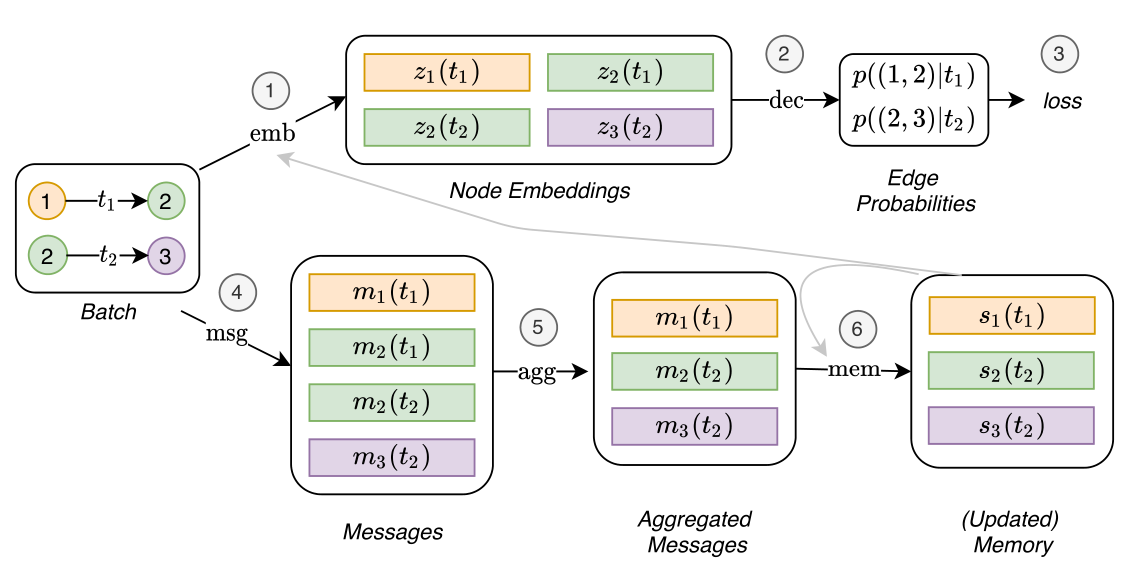
\includegraphics[width=0.65\textwidth,height=\textheight]{tgn_computations.png}
\caption{TGN computations on a single batch of time-stamped
interactions.}
\end{figure}

\[
\mathbf{m}_i(t) = \mathrm{msg}\left(\mathbf{s}_i(t^-), \mathbf{s}_j(t^-), \Delta t, \mathbf{e}_{ij}(t)\right)
\]
\end{frame}

\begin{frame}{Message aggregator}
\protect\hypertarget{message-aggregator}{}
\begin{figure}
\centering
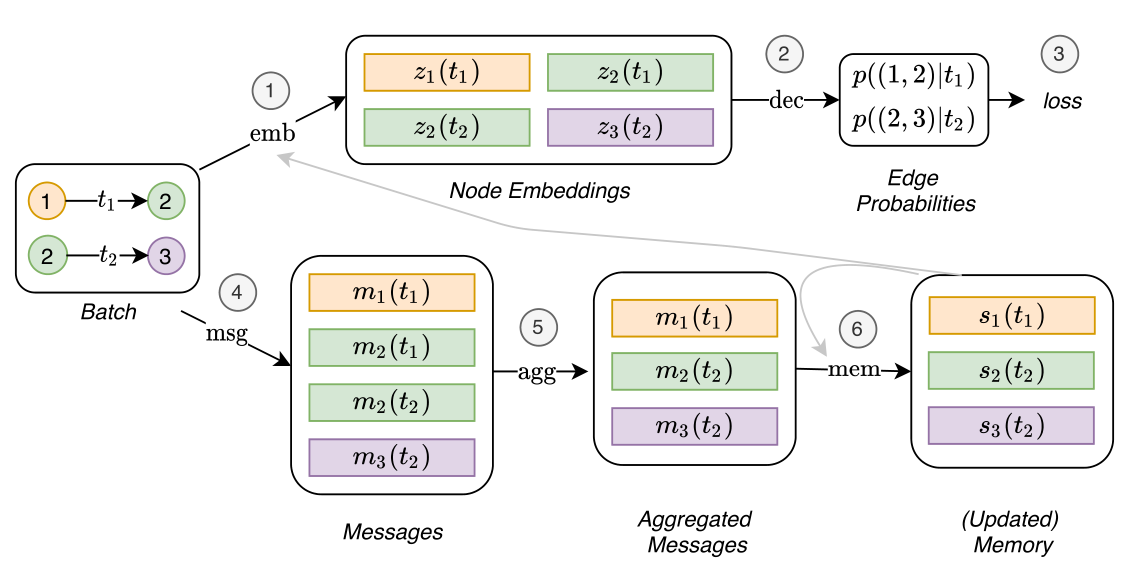
\includegraphics[width=0.65\textwidth,height=\textheight]{tgn_computations.png}
\caption{~}
\end{figure}

Combine all messages in a single batch for a specific node: \[
\bar{\mathbf{m}}_i(t) = \mathrm{agg}\left(\mathbf{m}_i(t_1), \hdots, \mathbf{m}_i(t_b)\right)
\]
\end{frame}

\begin{frame}{Memory update}
\protect\hypertarget{memory-update}{}
\begin{figure}
\centering
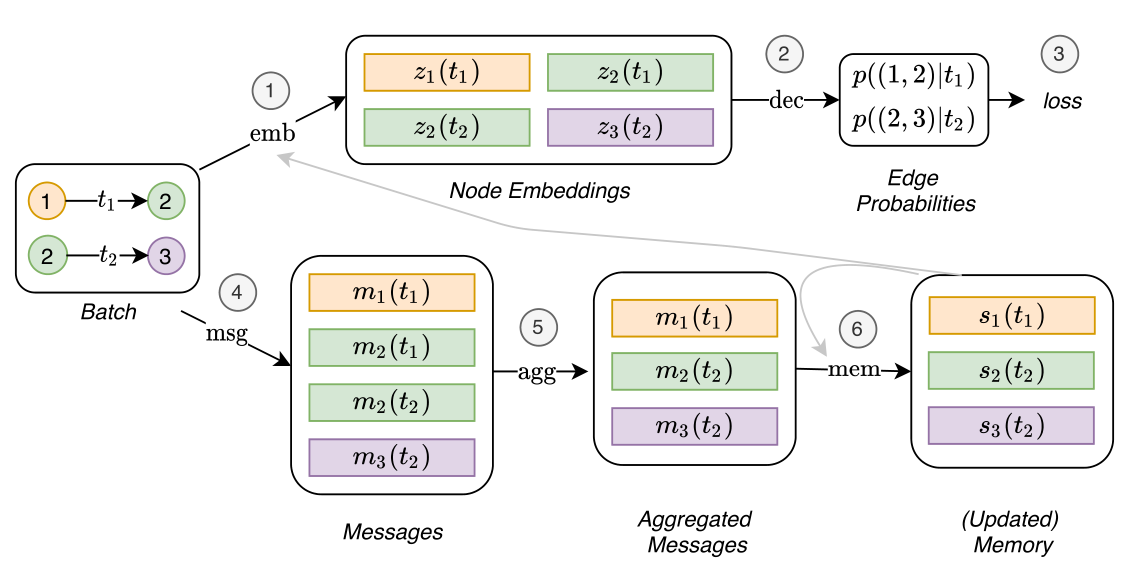
\includegraphics[width=0.65\textwidth,height=\textheight]{tgn_computations.png}
\caption{TGN computations on a single batch of time-stamped
interactions.}
\end{figure}

Using a Recurrent Neural Network: \[
\mathbf{s}_i(t) = \mathrm{mem}\left(\bar{\mathbf{m}}_i(t), \mathbf{s}_i(t^-)\right)
\]
\end{frame}

\begin{frame}{Embedding computation}
\protect\hypertarget{embedding-computation}{}
\begin{figure}
\centering
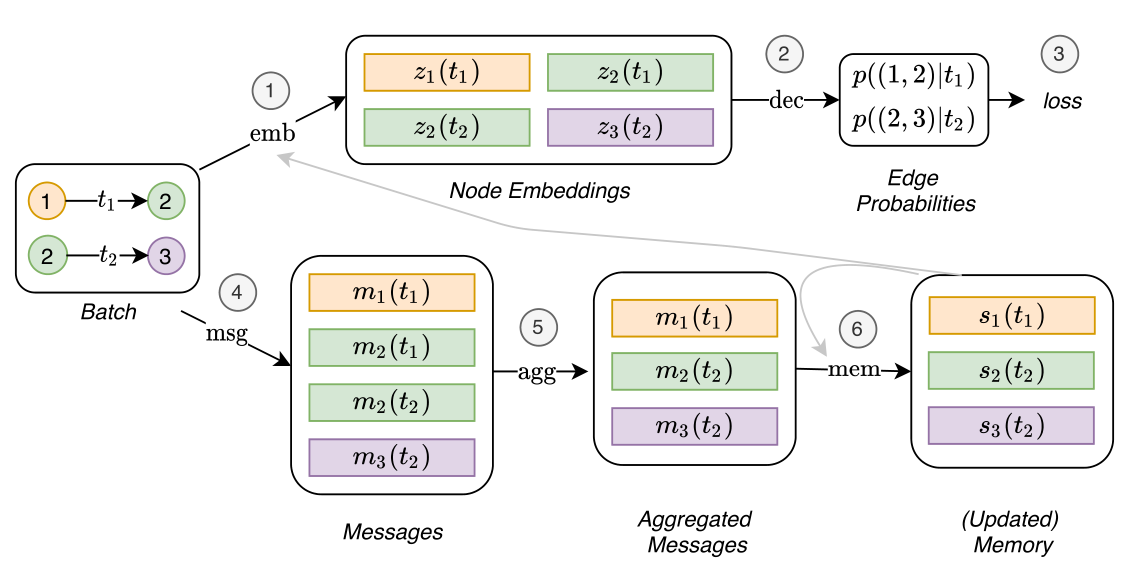
\includegraphics[width=0.65\textwidth,height=\textheight]{tgn_computations.png}
\caption{~}
\end{figure}

\[
\mathbf{z}_i(t) = \mathrm{emb}(i, t) = \sum_{j \in \mathcal{N}^k_i([0, t]) } h\left(\mathbf{s}_i(t), \mathbf{s}_j(t), \mathbf{e}_{ij}, \mathbf{v}_i(t), \mathbf{v}_j(t)\right), \nonumber
\]

Includes specific cases like: memory directly, time projection (JODIE),
Temporal Graph Attention (TGAT), Temporal Graph Sum
\end{frame}

\begin{frame}[fragile]{TGN training}
\protect\hypertarget{tgn-training}{}
\begin{figure}
\centering
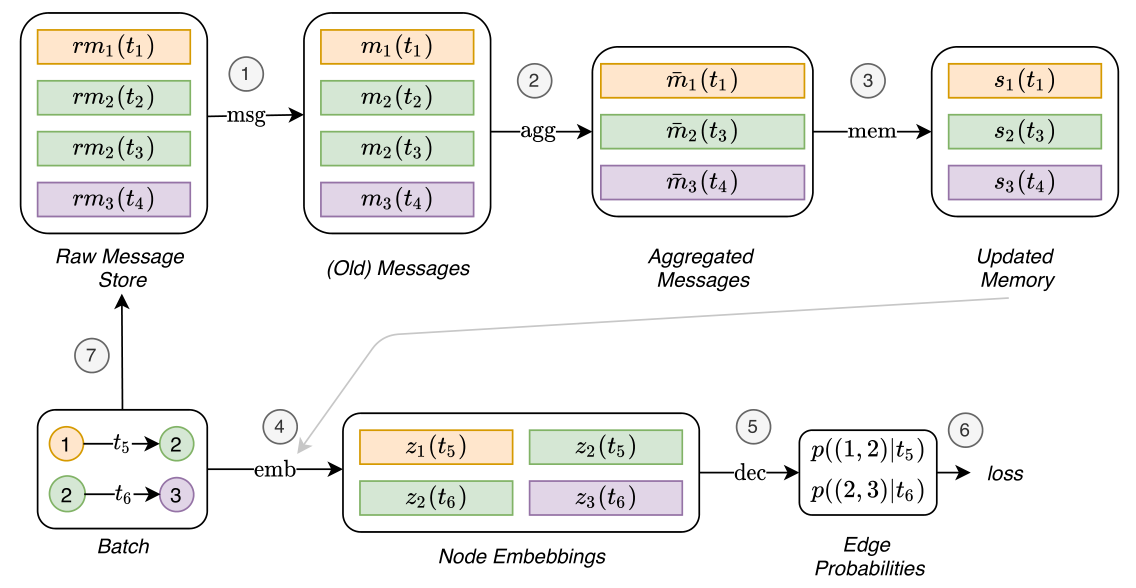
\includegraphics[width=0.65\textwidth,height=\textheight]{tgn_train.png}
\caption[TGN training ]{TGN training \footnotemark{}}
\end{figure}
\footnotetext{Figure taken from ``Temporal Graph Networks For Deep
  Learning on Dynamic Graphs, \emph{Rossi et al.}''

  \hypertarget{gdelt-dataset}{%
  \section{GDELT Dataset}\label{gdelt-dataset}}

  \hypertarget{the-gdelt-dataset}{%
  \subsection{The GDELT Dataset}\label{the-gdelt-dataset}}

  \begin{quote}
  ``The GDELT Project monitors the world's broadcast, print, and web
  news from nearly every corner of every country in over 100 languages
  and identifies the people, locations, organizations, themes, sources,
  emotions, counts, quotes, images and events driving our global society
  every second of every day, creating a free open platform for computing
  on the entire world.''
  \end{quote}

  \begin{itemize}
  \tightlist
  \item
    Global Knowledge Graph
  \item
    Global Event Database
  \item
    Global Entity Graph
  \item
    Global Frontpage Graph
  \end{itemize}

  \hypertarget{the-global-entity-graph}{%
  \subsection{The Global Entity Graph}\label{the-global-entity-graph}}

  Random sample of news articles every 15 minutes (roughly 100k per day)

  Google NLP API extracts entities from each article

\begin{Shaded}
\begin{Highlighting}[]
\FunctionTok{\{}
  \DataTypeTok{"url"}\FunctionTok{:} \StringTok{"https://chicago.suntimes.com/news/washington{-}state{-}ends{-}racially{-}biased{-}death{-}penalty/"}\FunctionTok{,}
  \DataTypeTok{"lang"}\FunctionTok{:} \StringTok{"en"}\FunctionTok{,}
  \DataTypeTok{"date"}\FunctionTok{:} \StringTok{"2018{-}10{-}12T00:15:00Z"}\FunctionTok{,}
  \DataTypeTok{"score"}\FunctionTok{:} \FloatTok{{-}0.2}\FunctionTok{,}
  \DataTypeTok{"magnitude"}\FunctionTok{:} \FloatTok{12.3}\FunctionTok{,}
  \DataTypeTok{"entities"}\FunctionTok{:} \OtherTok{[}
    \FunctionTok{\{}
      \DataTypeTok{"name"}\FunctionTok{:} \StringTok{"Supreme Court"}\FunctionTok{,}
      \DataTypeTok{"type"}\FunctionTok{:} \StringTok{"ORGANIZATION"}\FunctionTok{,}
      \DataTypeTok{"numMentions"}\FunctionTok{:} \DecValTok{1}\FunctionTok{,}
      \DataTypeTok{"avgSalience"}\FunctionTok{:} \FloatTok{0.04405}
    \FunctionTok{\}}\OtherTok{,}
    \ErrorTok{...}
\ErrorTok{\}}
\end{Highlighting}
\end{Shaded}

  \hypertarget{creating-a-graph}{%
  \subsection{Creating a Graph}\label{creating-a-graph}}

  Each pair of entities occurring in a single article correspond to an
  edge event with timestamp:

\begin{Verbatim}
Nathan Trott        RB Leipzig
Manchester United   RB Leipzig
West Ham            RB Leipzig
Timo Werner         RB Leipzig
Ralf Rangnick       RB Leipzig
Bundesliga          RB Leipzig
Patrick Dempsey     Leipzig
Leipzig             Germany
Patrick Dempsey     Leipzig
Leipzig             Germany
Patrick Dempsey     Leipzig
Leipzig             Germany
...
\end{Verbatim}

  Restricting to the 4 most salient entities gives roughly 200k edges
  per day

  \hypertarget{data-example-ipcc}{%
  \subsection{Data Example: IPCC}\label{data-example-ipcc}}

  \begin{columns}[T]
  \begin{column}{0.48\textwidth}
  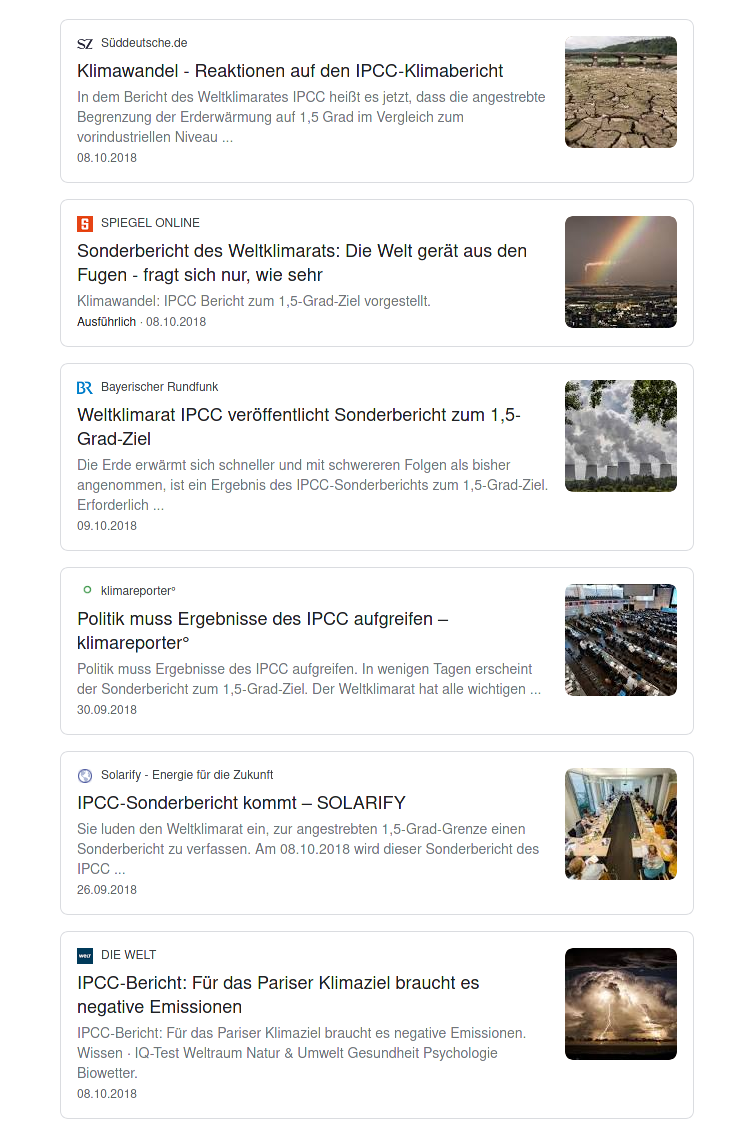
\includegraphics{ipcc_headlines.png}
  \end{column}

  \begin{column}{0.48\textwidth}
  \begin{figure}
  \centering
  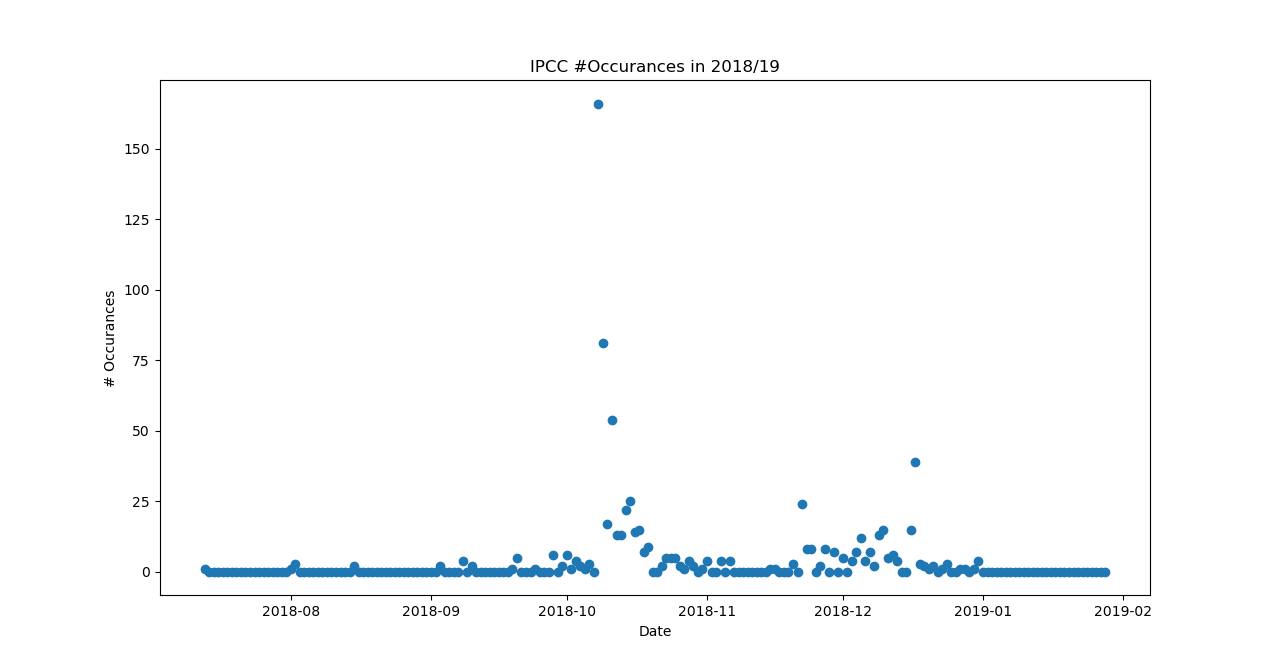
\includegraphics{ipcc_2018.png}
  \caption{\# Occurrences IPCC}
  \end{figure}

\begin{Verbatim}
         entity_1   entity_2  count
             IPCC      India     18
Michael McCormack       IPCC     15
   Scott Morrison       IPCC     15
            India       IPCC     15
     Donald Trump       IPCC     15
    United States       IPCC     14
   European Union       IPCC     14
      Hoesung Lee       IPCC     14
ottish Government       IPCC     12
             IPCC         US     12
\end{Verbatim}
  \end{column}
  \end{columns}}

Problem: memory-related modules (Message function, Message aggregator,
and Memory updater) do not directly influence the loss and therefore do
not receive a gradient -\textgreater{} memory update before predictions
\end{frame}

\hypertarget{research-idea}{%
\section{Research Idea}\label{research-idea}}

\begin{frame}{Motivation}
\protect\hypertarget{motivation}{}
\begin{block}{How can we identify entities with similar temporal
dynamics, e.g.~``hot'' topics?}
\protect\hypertarget{how-can-we-identify-entities-with-similar-temporal-dynamics-e.g.-hot-topics}{}
\end{block}
\end{frame}

\begin{frame}{Approach}
\protect\hypertarget{approach}{}
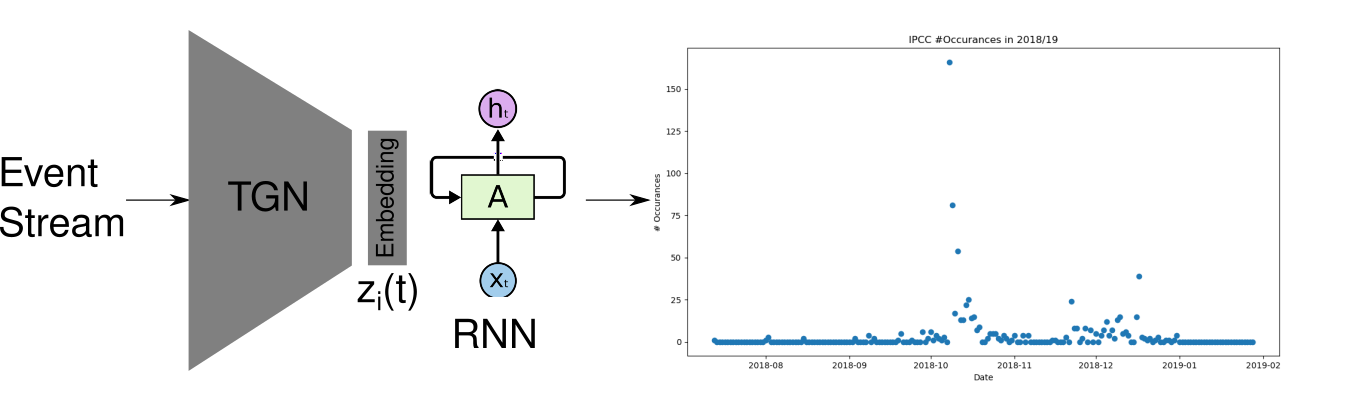
\includegraphics{motiviaton_arch.png}

Replace decoder with a RNN which predicts the future \#Occurrences per
day for a given entity and time horizon
\end{frame}

\begin{frame}{Approach}
\protect\hypertarget{approach-1}{}
\begin{columns}[T]
\begin{column}{0.48\textwidth}
\emph{Why is the graph information relevant?}

\begin{center}\rule{0.5\linewidth}{0.5pt}\end{center}

The neighborhood should be strong indicator for future behavior: If all
my neighbors are getting popular, then it is very likely that I will
too.

Example: If a footballer is mentioned during an event like a world cup,
it should be much more active.
\end{column}

\begin{column}{0.48\textwidth}
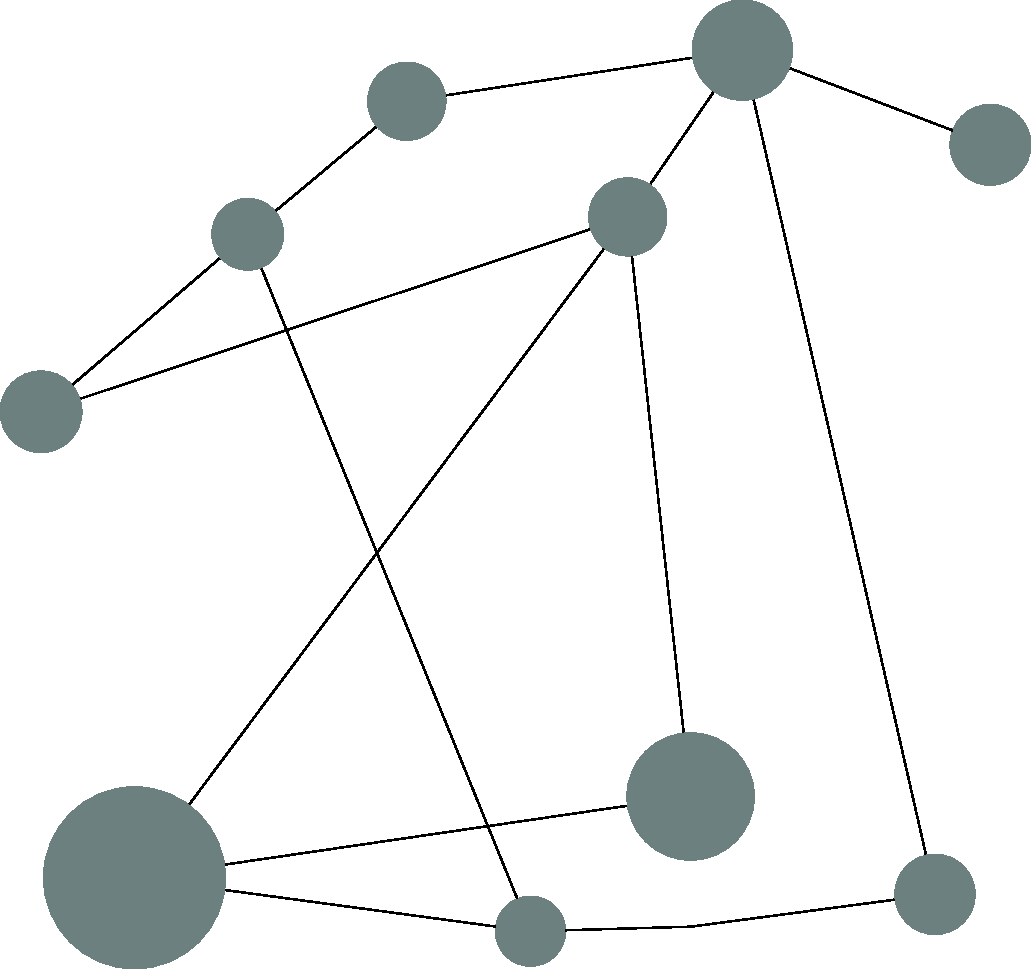
\includegraphics{graph_temp.pdf}
\end{column}
\end{columns}
\end{frame}

\begin{frame}{The Embedding Space}
\protect\hypertarget{the-embedding-space}{}
\begin{itemize}
\tightlist
\item
  before (link prediction): similarity predicts future link between two
  entities
\item
  now (activity prediction): embedding space represents temporal
  dynamics

  \begin{itemize}
  \tightlist
  \item
    clustering
  \item
    split relative and absolute dynamics
  \item
    duplicate detection
  \end{itemize}
\end{itemize}
\end{frame}

\begin{frame}{Challenges}
\protect\hypertarget{challenges}{}
Test
\end{frame}

\begin{frame}{Details}
\protect\hypertarget{details}{}
\begin{itemize}
\tightlist
\item
  Current state:

  \begin{itemize}
  \tightlist
  \item
    preparing dataset
  \end{itemize}
\item
  Baseline: time series prediction for number of occurrences (no
  neighborhood info)
\item
  Open questions:

  \begin{itemize}
  \tightlist
  \item
    What is a single data point?
  \item
    How to batch the data?
  \end{itemize}
\end{itemize}
\end{frame}

\end{document}
